% TO DO: add book covers, discuss SVI and LDA example, maybe simple Dutch book but not so easy, use regularized regression as a red rope, with horseshoe as right subjective prior but also right frequentist prior provided EB is used to estimate the number of nonzero components.

\documentclass[10pt]{beamer}
\usetheme[height=0mm]{Rochester}
\usefonttheme[onlylarge]{structurebold}
\setbeamerfont*{frametitle}{size=\normalsize,series=\bfseries}
\setbeamertemplate{navigation symbols}{}
\setbeamercovered{dynamic}
\setbeamertemplate{itemize item}[triangle]
\setbeamertemplate{itemize subitem}[triangle]
%\useoutertheme{infolines}

%  use Darmstadt if commenting the next line
\usepackage[footheight=1em]{beamerthemeboxes}
\usepackage[natbib=true,backend=biber,citestyle=authoryear]{biblatex}
\bibliography{stats,../bib/stats,../bib/learning}

\usepackage{amsmath,amssymb,amsthm,bbm}             % AMS Math
\usepackage[utf8]{inputenc}
\usepackage[english]{babel}
\usepackage{myAlgorithm}
\usepackage{xcolor}
\usepackage{graphicx}
\usepackage{subfigure}
\usepackage{hyperref}
\usepackage{mathtools}
\usepackage{mathrsfs}
\usepackage{wasysym}
\usepackage{tikz}
\usetikzlibrary{bayesnet}
\usetikzlibrary{arrows}
\usepackage{url}

% notation
\DeclareMathOperator*{\argmax}{arg\,max}
\DeclareMathOperator*{\argmin}{arg\,min}
\newcommand{\cA}{\mathcal{A}}
\newcommand{\cS}{\mathcal{S}}
\newcommand{\cF}{\mathcal{F}}
\newcommand{\cX}{\mathcal{X}}
\newcommand{\cY}{\mathcal{Y}}
\newcommand{\cZ}{\mathcal{Z}}
\newcommand{\cN}{\mathcal{N}}
\newcommand{\cO}{\mathcal{O}}
\renewcommand{\leq}{\leqslant}
\renewcommand{\geq}{\geqslant}
\renewcommand{\phi}{\varphi}
\renewcommand{\epsilon}{\varepsilon}
\renewcommand{\d}{ {\rm d}}
\renewcommand{\emptyset}{\varnothing}

\newcommand\un[1]{\textcolor{magenta}{#1}}
\newcommand\unn[1]{\textcolor{blue}{#1}}
\newcommand\unnn[1]{\textcolor{red}{#1}}
\newcommand\unnnn[1]{\textcolor{orange}{#1}}

\def\cX{\mathcal{X}}
\def\cY{\mathcal{Y}}
\def\cZ{\mathcal{Z}}
\def\cS{\mathcal{S}}
\def\cR{\mathcal{R}}
\def\cA{\mathcal{A}}

\def\by{\mathbf{y}}

% indicator
\newcommand\IND[1]{\mathbbm{1}_{\{#1\}}}

\def\cfdemo{\url{https://chi-feng.github.io/mcmc-demo/}}

\def\tpi{\widetilde{\pi}}
\def\cN{\mathcal{N}}
\renewcommand\d{\mathrm{d}}
\def\e{\mathrm{e}}

\usecolortheme[named=bleu]{structure}

\title[Bayesian ML: what, why, and how?]{Bayesian ML: what, why, and how?}
\subtitle{Part \#1: what is Bayesian ML?}
\author[Rémi Bardenet (CNRS \& Univ. Lille)] % (optional, for multiple authors)
{Rémi Bardenet}
\institute[] % (optional)
{
  CNRS \& CRIStAL, Univ. Lille, France\\
\vspace{1cm}

\includegraphics[width=0.15\textwidth]{Logos/logo_CNRS.pdf}
\qquad \includegraphics[width=0.35\textwidth]{Logos/logo_CRISTAL}
\qquad
\includegraphics[width=0.15\textwidth]{Logos/logo_ERC}
\qquad 
\includegraphics[width=0.13\textwidth]{Logos/logo_funded_by_ANR}
}
\date{}

\begin{document}
\begin{frame}
\maketitle
\end{frame}

\begin{frame}{Make sure you're in the right class}
\begin{center}
  \includegraphics[width=\onefig]{Figures/bodybuilding}
\end{center}
\end{frame}
 
\begin{frame}
  \frametitle{These are more the applications we have in mind}
  \only<1>{
  \fbox{
    
\includegraphics[trim={0 15cm 0 0},clip,width=\textwidth]{Papers/virgo.pdf}
  }
  }
  \only<2>{
  \fbox{
    \includegraphics[trim={0 3cm 0 12cm},clip,width=\textwidth]{Figures/virgop4.pdf}
  }
  }
\end{frame}

\begin{frame}{or that one}
\only<1>{
  \fbox{
    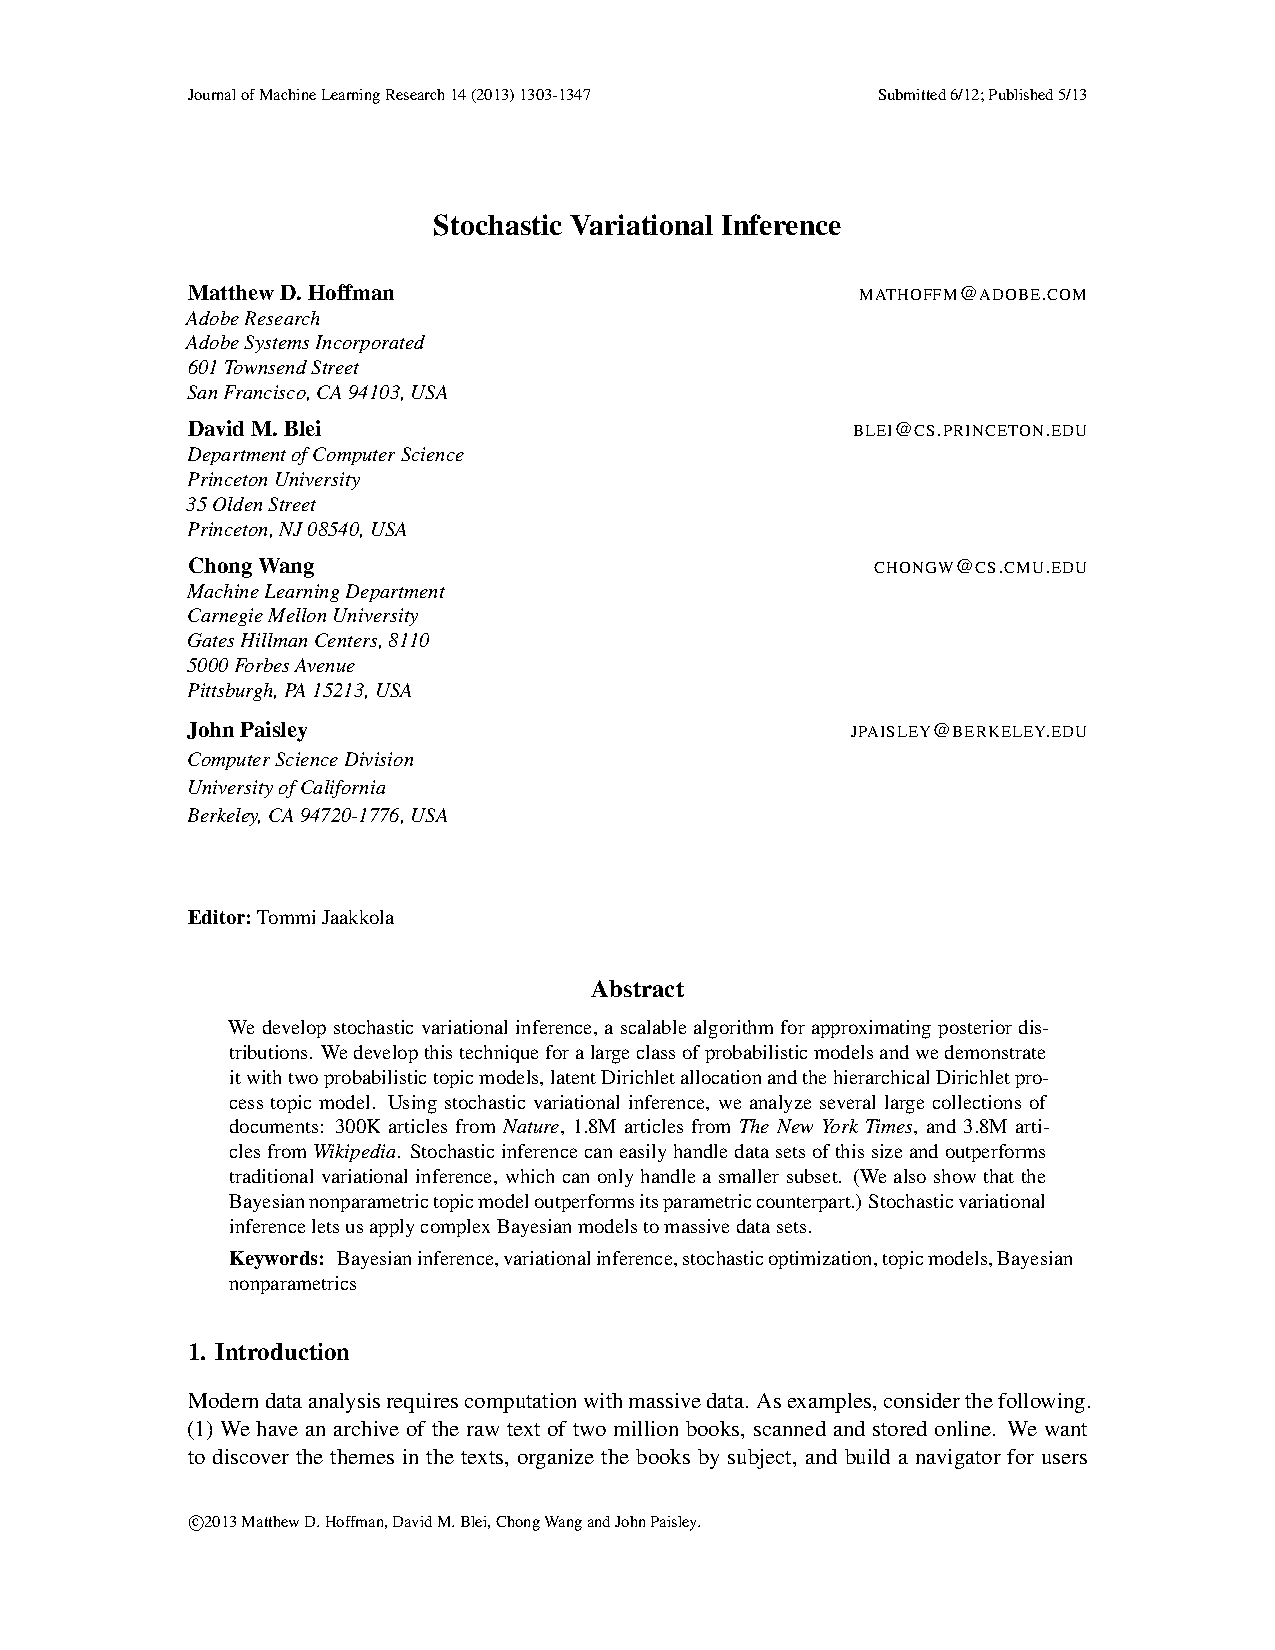
\includegraphics[trim={0cm 15cm 0 0},clip,width=\textwidth]{Papers/svi.pdf}
  }
}
\only<2>{
  \frametitle{or that one}
  \fbox{
    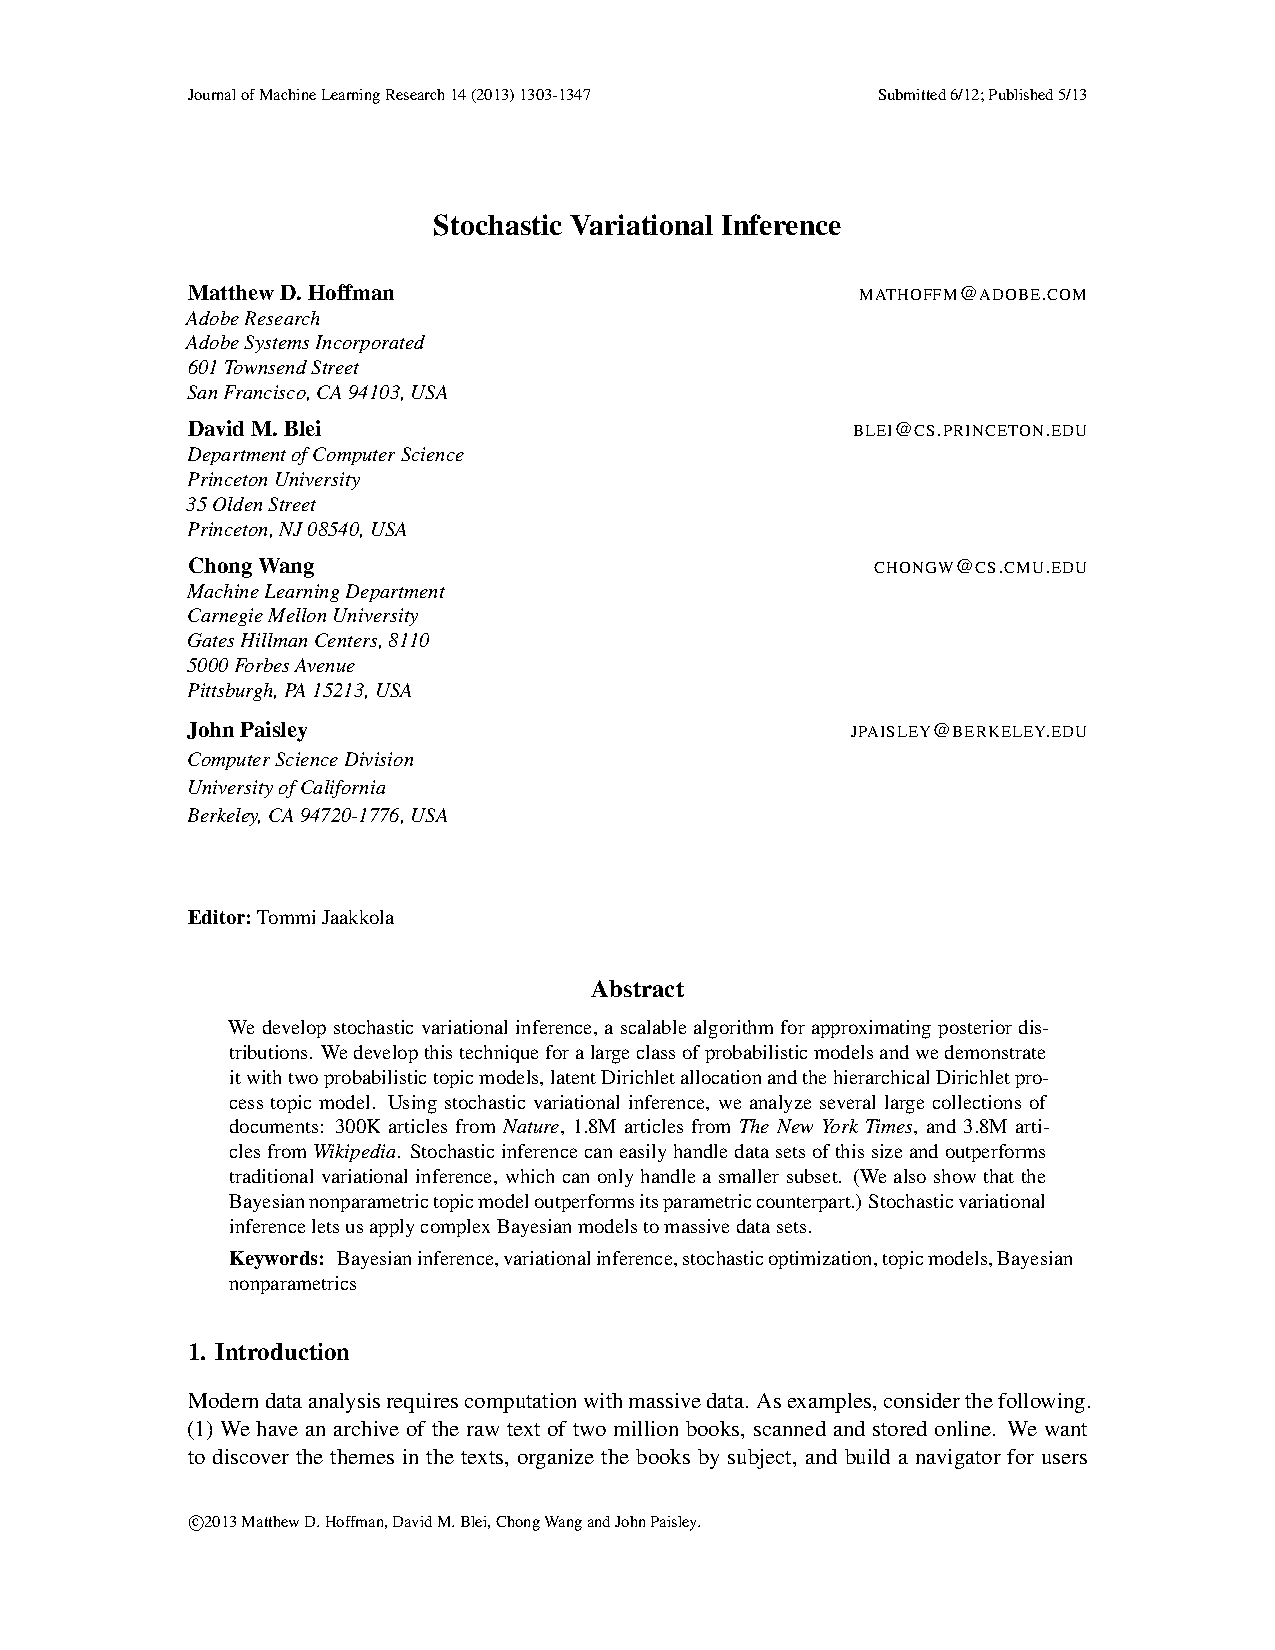
\includegraphics[trim={0cm 0 0 15cm},clip,width=\textwidth]{Papers/svi.pdf}
  }
}
\end{frame}

\begin{frame}
\frametitle{Outline}
\tableofcontents
\end{frame}

\section{A data-driven definition}
\begin{frame}
  \frametitle{Bayesian keywords in NeurIPS abstracts, up to 2016}
  \begin{figure}
    \subfigure[``Bayesian" at NeurIPS]{
    \includegraphics[width=\twofig]{Figures/bayesianPapersNIPS.pdf}
    \label{f:papers:BayesianNeurIPS}
    }
    \subfigure[``Neural net" at NeurIPS]{
    \includegraphics[width=\twofig]{Figures/neuralPapersNIPS.pdf}
    \label{f:papers:NNNeurIPS}
    }
    \label{f:papers}
    %\caption{Trends for papers appearing in JMLR and at NeurIPS, up to 2016.}
\end{figure}
\end{frame}

\begin{frame}
  \frametitle{Topics automatically extracted from 1000+ ``Bayesian" abstracts}
  \begin{figure}
    \footnotesize
    \begin{tabular}{|l|}
    \hline
      \textcolor{vert}{model models data process latent Bayesian Dirichlet hierarchical nonparametric inference}\\
      features learn problem different knowledge learning image object example examples\\
      method neural Bayesian using linear state based kernel approach model\\
      belief propagation nodes local tree posterior node nbsp given algorithm\\
      learning data Bayesian model training classification performance selection prediction sets\\
      \textcolor{bleu}{inference Monte Carlo Markov sampling variational time algorithm MCMC approximate}\\
      function optimization algorithm optimal learning problem gradient methods bounds state\\
      learning networks variables structure network Bayesian EM paper distribution algorithm\\
      \textcolor{magenta}{Bayesian gaussian prior regression non estimation likelihood sparse parameters matrix}\\
      model information Bayesian human visual task probability sensory prior concept\\
    \hline
    \end{tabular}
    \caption{Topics extracted by stochastic variational latent Dirichlet allocation, using {scikit-learn} \citep{sklearn11}.
    \label{f:bayesianTopics}}
    \end{figure}
\end{frame}

\section{A warmup: Estimation in regression models}

\begin{frame}{A recap on probabilistic graphical models \citep[Section 10.5]{Mur12}}
  \begin{itemize}
    \item PGMs (aka ``Bayesian" networks) represent the dependencies in a joint distribution $p(s)$ by \un{a directed graph $G=(E,V)$}.
    \item Two important properties:
    $$
    p(s) = \prod_{v\in V} p(s\vert s_{\text{pa(v)}}) \qquad\text{and}\qquad
    s_v \perp s_{nd(v)\setminus pa(v)} \vert s_{pa(v)}.
    $$
  \end{itemize}
  \blank
\end{frame}


\begin{frame}{Inference in regression models}
\vspace{-1.5cm}
\begin{flushright}
  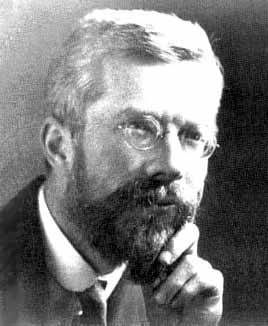
\includegraphics[width=\threefig]{Figures/fisher.jpg}
\end{flushright}
\vfill 
\end{frame}

\begin{frame}{Inference in regression models}
  \vspace{-1.5cm}
  \begin{flushright}
    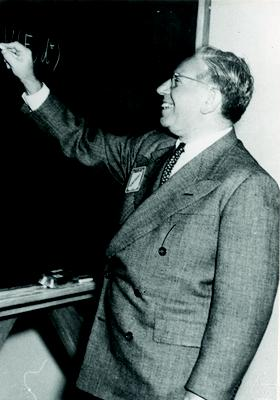
\includegraphics[width=\threefig]{Figures/wald2}
  \end{flushright}
  \vfill 
\end{frame}

\begin{frame}{Inference in regression models}
  \vspace{-1.5cm}
  \begin{flushright}
    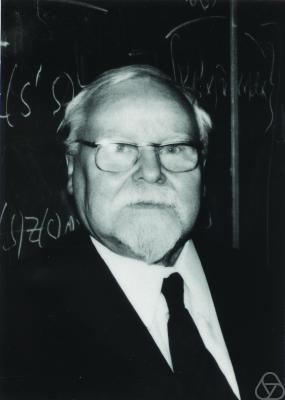
\includegraphics[width=\threefig]{Figures/tykhonov.jpg}
  \end{flushright}
  \vfill 
\end{frame}

\begin{frame}{Inference in regression models}
  \vspace{-1.5cm}
  \begin{flushright}
    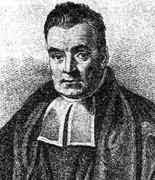
\includegraphics[width=\threefig]{Figures/bayes}
  \end{flushright}
  \vfill 
\end{frame}

\begin{frame}{Inference in regression models}
\end{frame}

% \begin{frame}
%   \frametitle{Classification as a decision problem}
% \end{frame}

% \begin{frame}
%   \frametitle{A quick motivating example before we go formal 1/2}
%   \begin{itemize}
%     \vfill\item Let $N$ individuals evolve from Susceptible to Infected to Recovered, $x_n(t) \in\{S,I,R\}$, $1\leq n\leq N$, $t\in[0,T]$.
%     \vfill\item Each susceptible individual $n$ moves to $R$ according to a Poisson process with intensity
%     $$\sum_{k:x_k(t)=I} \lambda_{nk}(\unn{\theta_{SI}}).$$
%     \vfill\item Each infected person recovers after a Gamma(\unn{$a,b$}) time.
%     \vfill\item This allows to express
%     $$
%     p(x_1(t_{1,1}), \dots, x_1(t_{1,T_1}), \cdots, x_n(t_{n,1}), \dots, x_1(t_{n,T_n})\vert \unn{\theta}).
%     $$
%     where \unn{$\theta= (\theta_{SI}, a, b)$}.
%     \vfill\item Now, consider $p(\theta\vert \text{data}) \propto p(\text{data}\vert \theta) \un{p(\theta)}.$
%   \end{itemize}
% \end{frame}

% \begin{frame}
% \frametitle{A quick motivating example before we go formal 2/2}
%   \begin{itemize}
%   \vfill\item If asked to report an interval on a particular function of $\theta$, say $R_0$, I would output a small interval $I$ such that
%   $$ \int_I p(\theta\vert \text{data}) \,\d\theta \geq 0.95.$$
%   \vfill\item If asked whether we should close universities, I would ask for
%   \begin{itemize}
%     \item \un{the cost $\alpha$ of closing unis when $R_0<1$},
%     \item \unn{the cost $\beta$ of keeping unis open while $R_0>1$}.
%   \end{itemize}
%   \vfill\item Then I would recommend closing if and only if
%   $$
%   p(R_0>1\vert \text{data}) > \frac{\un{\alpha}}{\un{\alpha}+\unn{\beta}}.
%   $$
%   \vfill\item Additionally, I would check that the decision doesn't change if I change my prior $p(\theta)$ a little.
%   \vfill\item If it did, then I would refine my likelihood and/or wait for more data.
% \end{itemize}

% \tikz{ %
  %   \node[latent] (S) {$S$};%
  %   \node[latent,right=of S] (I) {$I$}; %
  %   \node[latent,right=of I] (R) {$R$}; %
  %   \edge S I;
  %   \edge I R;
  % }
% \end{frame}

% \begin{frame}{Quotes from \citep{GCSDVR13} on Bayesian methods}
% % put book picture
% \begin{itemize}
%  \vfill\item \emph{[...] practical methods for making inferences from data, using probability models for quantities we observe \un{and for quantities about which we wish to learn}.}
% \vfill\item \emph{The essential characteristic of Bayesian methods is their \un{explicit use of probability for quantifying uncertainty} in inferences based on statistical data analysis.}
% \vfill\item \emph{Three steps:
% \begin{enumerate}
%   \item Setting up a full probability model,
%   \item Conditioning on observed data, calculating and interpreting the appropriate ``posterior distribution",
%   \item Evaluating the fit of the model and the implications of the resulting posterior distribution. In response, one can alter or expand the model and repeat the three steps.
% \end{enumerate}
% }
% \end{itemize}
% \end{frame}

% \begin{frame}{Notation that I will try to stick to}
% \begin{itemize}
%   \vfill\item $y_{1:n} = (y_1,\dots,y_n) \in \cY^n$ denote observable data/labels.
%   \vfill\item $x_{1:n} \in \cX^n$ denote covariates/features/hidden states.
%   \vfill\item $z_{1:n} \in \cZ^n$ denote hidden variables.
%   \vfill\item $\theta\in\Theta$ denote parameters.
%   \vfill\item $X$ denotes an $\cX$-valued random variable. Lowercase $x$ denotes either a point in $\cX$ or an $\cX$-valued random variable.
% \end{itemize}
% \end{frame}

% \begin{frame}{More notation}
%   \begin{itemize}
%   \vfill\item Whenever it can easily be made formal,
%   %(by choosing an appropriate reference $\sigma$-finite measure, say Lebesgue or the counting measure),
%   we write densities for our random variables and let the context indicate what is meant. So if $X\sim \cN(0,\sigma^2)$, we write
%   $$ \mathbb E h(X) = \int h(x) \frac{e^{-x^2/2\sigma^2}}{\sigma\sqrt{2\pi}}\d x = \int h(x)p(x)\mathrm{d}x.$$
%   Similarly, for $X\sim \mathcal P(\lambda)$, we write
%   $$ \mathbb E h(X) = \sum_{k=0}^\infty h(k) e^{-\lambda}\frac{\lambda^k}{k!} = \int h(x) p(x)\mathrm{d} x$$
%   \vfill\item All pdfs are denoted by $p$, so that, e. g.
%   \begin{align*}
% \mathbb{E} h(Y, \theta) &= \int h(y, \theta)p(y, \theta)\,\d y\d \theta\\
% &= \int h(y, \theta)p(y, x, \theta) \,\d x\d y \d\theta\\
% &= \int h(y, \theta) p(y, \theta\vert x)p(x) \,\d x\d y \d\theta
%   \end{align*}
% \end{itemize}

% \end{frame}

\section{ML as data-driven decision-making}

\begin{frame}{Describing a decision problem under uncertainty \citep{Wal50}}
\begin{itemize}
  \vfill\item A state space $\cS$,\\
  \un{Every quantity you need to consider to make your decision.}
  \vfill\item Actions $\cA \subset \cF(\cS, \cZ)$,\\
  \un{Making a decision means picking one of the available actions.}
  \vfill\item A reward space $\cZ$,\\
  \un{Encodes how you feel about having picked a particular action.}
  \vfill\item A loss function $L:\cA\times \cS \rightarrow \mathbb{R}_+$.\\
  \un{How much you would suffer from picking action $a$ in state $s$. 
  %It is also customary to first define a utility $u:\cZ\rightarrow \mathbb{R}_+$, and then let
  %$$ L(a,s) = \sup_{a'\in\cA} u\big(a'(s)\big) - u\big(a(s)\big) \in\mathbb{R}_+.$$
  }
\end{itemize}
\end{frame}

% \begin{frame}{Estimation as a decision problem}
%   \begin{itemize}
%   \item $\cS = $
%   \item $\cZ = $
%   \item $\cA = $
%   \item
%   \end{itemize}
%   \blank
% \end{frame}

\begin{frame}{Classification as a decision problem}
\begin{itemize}
\item $\cS = \un{\cX^n\times\cY^n}\times \cX\times \cY$, i.e. $s = (x_{1:n}, y_{1:n}, x, y)$.
\item $\cZ = \{0,1\}$.
\item $\cA = \{a_g: s\mapsto 1_{y\neq g(x; \un{x_{1:n}, y_{1:n}})}, \quad g\in\mathcal{G}\}$.
\item $L(a_g,s) = 1_{y\neq g(x; \un{x_{1:n}, y_{1:n}})}$.
\end{itemize}
\vfill
\begin{block}{PAC bounds; see e.g. \citep{ShBe14}}
Let $(x_{1:n},y_{1:n})\sim \mathbb{P}^{\otimes n}$, and independently $(x,y)\sim \mathbb{P}$, we want an algorithm $g(\cdot; x_{1:n}, y_{1:n})\in\mathcal G$ such that if $n\geq n(\delta,\epsilon)$,
$$
\un{\mathbb{P}^{\otimes n}}\left[\mathbb{E}_{(x,y)\sim \mathbb P} L(a_g,s) \leq \epsilon\right] \geq 1-\delta.
$$
\end{block}\end{frame}

% \begin{frame}{Regression as a decision problem}
%   \begin{itemize}
%   \item $\cS = $
%   \item $\cZ = $
%   \item $\cA = $
%   \item
%   \end{itemize}
%   \blank
% \end{frame}

% \begin{frame}{Model choice as a decision problem}
%     \begin{itemize}
%       \item $\cS = $
%       \item $\cZ = $
%       \item $\cA = $
%       \item
%       \end{itemize}
%       \blank
%     \end{frame}

% \begin{frame}{Topic modeling as a decision problem}
%     \begin{itemize}
%        \item $\cS = $
%        \item $\cZ = $
%        \item $\cA = $
%        \item
%     \end{itemize}
%     \blank
% \end{frame}
        
% Regression, classification, estimation, dimensionality reduction, clustering, topic modelling as a more complex hidden variable model: gives states and losses, maybe state the main non-Bayesian solution.

\section{Subjective expected utility}
% State the principle, insist on the choice of p, comment on BDA.
% Recap on graphical models
% List all previous examples and show a graphical model and the Bayes action.
% Solve a few examples, link with non-Bayesian solutions like regularized regression. Horseshoe?
% Confront with preconceived ideas on BML. Insist that on top of being a general, interpretable principle, SEU is usually good for non-Bayesians too: BvM, smaller MSE, PAC-Bayes (to come). Moreover, philosophical support (also to come in lecture on foundations).
\begin{frame}{SEU is what defines the Bayesian approach}
\begin{block}{The subjective expected utility principle}
\begin{enumerate}
\item \un{Choose} $\cS, \cZ, \cA$ and a loss function $L(a,s)$,
\item \un{Choose} a distribution $p$ over $\cS$,
\item Take the corresponding \un{Bayes action}
\begin{equation}
a^\star \in \argmin_{a\in\mathcal{A}} \mathbb{E}_{s\sim p} L(a,s).
\label{e:seu}
\end{equation}
\end{enumerate}
\end{block}
\vfill

\begin{block}{Corollary: minimize the posterior expected loss}
If we partition $s=(s_{o}, s_{\text{u}})$, then
$$ a^\star \in \argmin_{a\in\mathcal{A}} \mathbb{E}_{s_{o}} \mathbb{E}_{s_{\text{u}}\vert s_{o}} L(a,s).$$
Equivalently to \eqref{e:seu}, given $s_o$, we choose
$$
a^\star = \delta(s_o) = \argmin_{a\in\mathcal{A}} \un{\mathbb{E}_{s_{\text{u}}\vert s_{o}} L(a,s)}.$$
\end{block}
\end{frame}

\section{Revisiting examples}

\begin{frame}{Estimation as a decision problem: point estimates}
  \begin{itemize}
    \item $\cS = \un{\cY^n}\times \Theta$.
    \item $\cZ = \Theta$.
    \item $\cA = \{a_g: s\mapsto \theta - g(y_{1:n})\}$.
    \item $L(a_g,s) = \Vert \theta - g(y_{1:n}) \Vert^2$.
    \end{itemize}
    \blank
    \vfill
\end{frame}

\begin{frame}{Estimation as a decision problem: credible intervals}
  \begin{itemize}
    \item $\cS = \un{\cY^n}\times \Theta$.
    \item $\cZ = \Theta$.
    \item $\cA = \{a_g: s\mapsto (1_{\theta \in g(y_{1:n})}, \vert g(y_{1:n})\vert) \}$.
    \item $L(a_g,s) = 1_{\theta \in g(y_{1:n})} + \gamma \vert g(y_{1:n})\vert$.
    \end{itemize}
    \blank
    \vfill
\end{frame}

% \begin{frame}{Topic modeling}
%   \begin{figure}
%     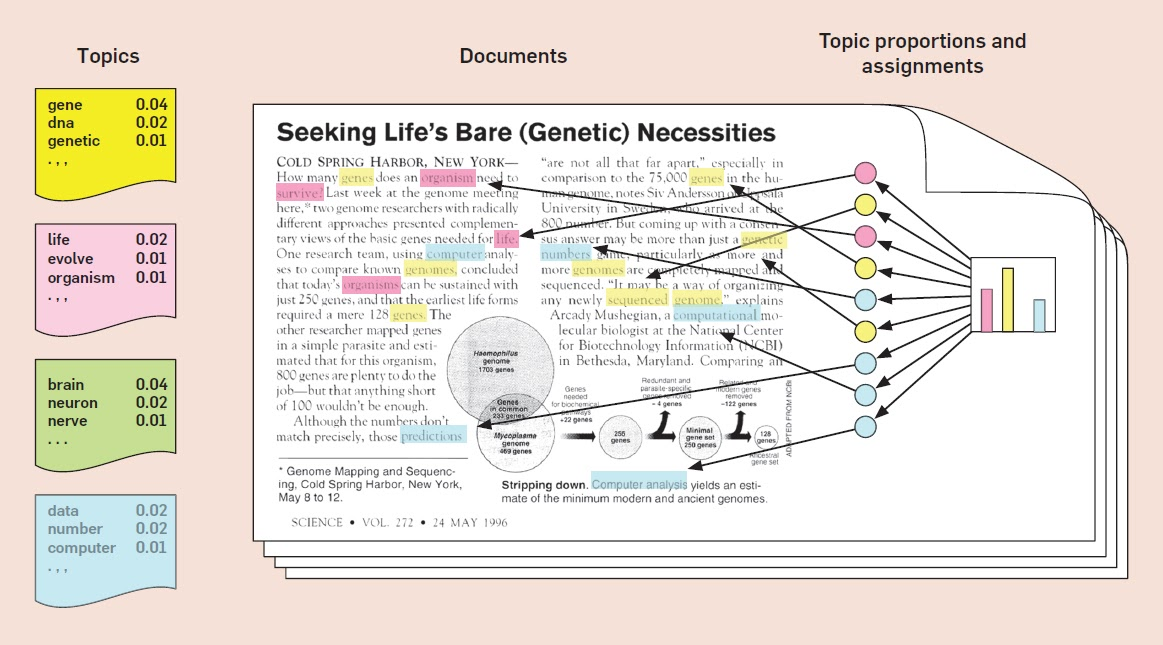
\includegraphics[width=\onefig]{Figures/lda.jpg}
%   \caption{Topic modeling. \emph{Credits to D. Blei?}}
%   \end{figure}
% \end{frame}

% \begin{frame}{Topic modelling as a decision problem}
%   \begin{itemize}
%     \item $\cS = $
%     \item $\cZ = $
%     \item $\cA = $
%     \item $L(a_g,s) = $
%     \end{itemize}
%     \blank
%     \vfill
%   \end{frame}

\begin{frame}{Classification as a decision problem}
  \begin{itemize}
    \item $\cS = \un{\cX^n\times\cY^n}\times \cX\times \cY \times \Theta$, i.e. $s = (x_{1:n}, y_{1:n}, x, y)$.
    \item $\cZ = \{0,1\}$.
    \item $\cA = \{a_g: s\mapsto 1_{y\neq g(x; \un{x_{1:n}, y_{1:n}})}\}$.
    \item $L(a_g,s) = 1_{y\neq g(x; \un{x_{1:n}, y_{1:n}})}$.
    \end{itemize}
    \blank
    \vfill
\end{frame}

\begin{frame}{Classification as a decision problem }
  \begin{itemize}
    \item $\cS = \un{\cX^n\times\cY^n}\times \cX\times \cY$, i.e. $s = (x_{1:n}, y_{1:n}, x, y)$.
    \item $\cZ = \{0,1\}$.
    \item $\cA = \{a_g: s\mapsto 1_{y\neq g(x; \un{x_{1:n}, y_{1:n}})}\}$.
    \item $L(a_g,s) = \un{\alpha 1_{y\neq g(x)} 1_{y = 0} + \beta 1_{y\neq g(x)} 1_{y = 1}}$.
    \end{itemize}
    \blank
    \vfill
\end{frame}

% \begin{frame}{Prediction in regression as a decision problem}
% % Exercise: Gaussian-Gaussian model, smaller MSE as an example of having good frequentist properties
% \begin{itemize}
%   \item $\cS = \un{\cX^n\times\mathbb{R}^n}\times \cX\times \mathbb{R}$, i.e. $s = (x_{1:n}, y_{1:n}, x, y)$.
%   \item $\cZ = \mathbb{R}$.
%   \item $\cA = \{a_g: s\mapsto y - g(x; \un{x_{1:n}, y_{1:n}})\}$.
%   \item $L(a_g,s) = \Vert y - g(x; \un{x_{1:n}, y_{1:n}}) \Vert^2$.
%   \end{itemize}
%   \blank
%   \vfill
% \end{frame}

% \begin{frame}{Dimensionality reduction as a decision problem}
% \end{frame}

% \begin{frame}{Clustering as a decision problem}
% \end{frame}


% \begin{frame}{Image denoising as a decision problem}
% % Find better example? Use one from Phuong's thesis?
% \begin{figure}
% \includegraphics[width=\textwidth]{Figures/denoising.png}
% \caption{Taken from \citep[Chapter 21]{Mur12}}
% \end{figure}
% \blank
% \end{frame}

\begin{frame}{Wrapping up}
  \begin{block}{A Bayesian minimizes a posterior expected loss}
  $$
    a^\star = \delta(s_o) = \argmin_{a\in\mathcal{A}} \un{\mathbb{E}_{s_{\text{u}}\vert s_{o}} L(a,s)}.
  $$
  \end{block}
  \vfill
  \begin{itemize}
    \item SEU allows to formalize most ML questions.
    \item Choosing $L$ and (the dependencies in) $\pi$ is often relatively natural.
    \item Everything boils down to integrals.
  \end{itemize}
  \vfill
  \begin{alertblock}{Good's {\it 46656 varieties of Bayesians}}
    \begin{itemize}
      \item Bayesian subschools differ on how they justify, interpret, and implement that principle.
      \item Different interpretations lead to different degrees of freedom for the joint model.
    \end{itemize}
  \end{alertblock}
  
% % \begin{block}{A few divisive questions}
% % \begin{itemize}
% % \item Using data or the likelihood to choose your prior; see Lecture \#5.
% % \item Using MAP estimators for their computational tractability, like in inverse problems
% % $$ \hat x_\lambda \in \argmin \Vert y- Ax\Vert + \lambda\Omega(x).$$
% % \item When and how should you revise your model (likelihood or prior)?
% % \item MCMC vs variational Bayes (more in Lectures \#2 and \#3)
% % \end{itemize}
% \end{block}
\end{frame}

\nocite{MaRo07,PaIn09,Rob07}

\section*{References}
\setbeamertemplate{bibliography item}[text]%,
\begin{frame}[allowframebreaks]
\frametitle{References}
\small
\printbibliography
\normalsize
\end{frame}
\end{document}
